\section{\name Design}
\begin{figure*}[htbp]
    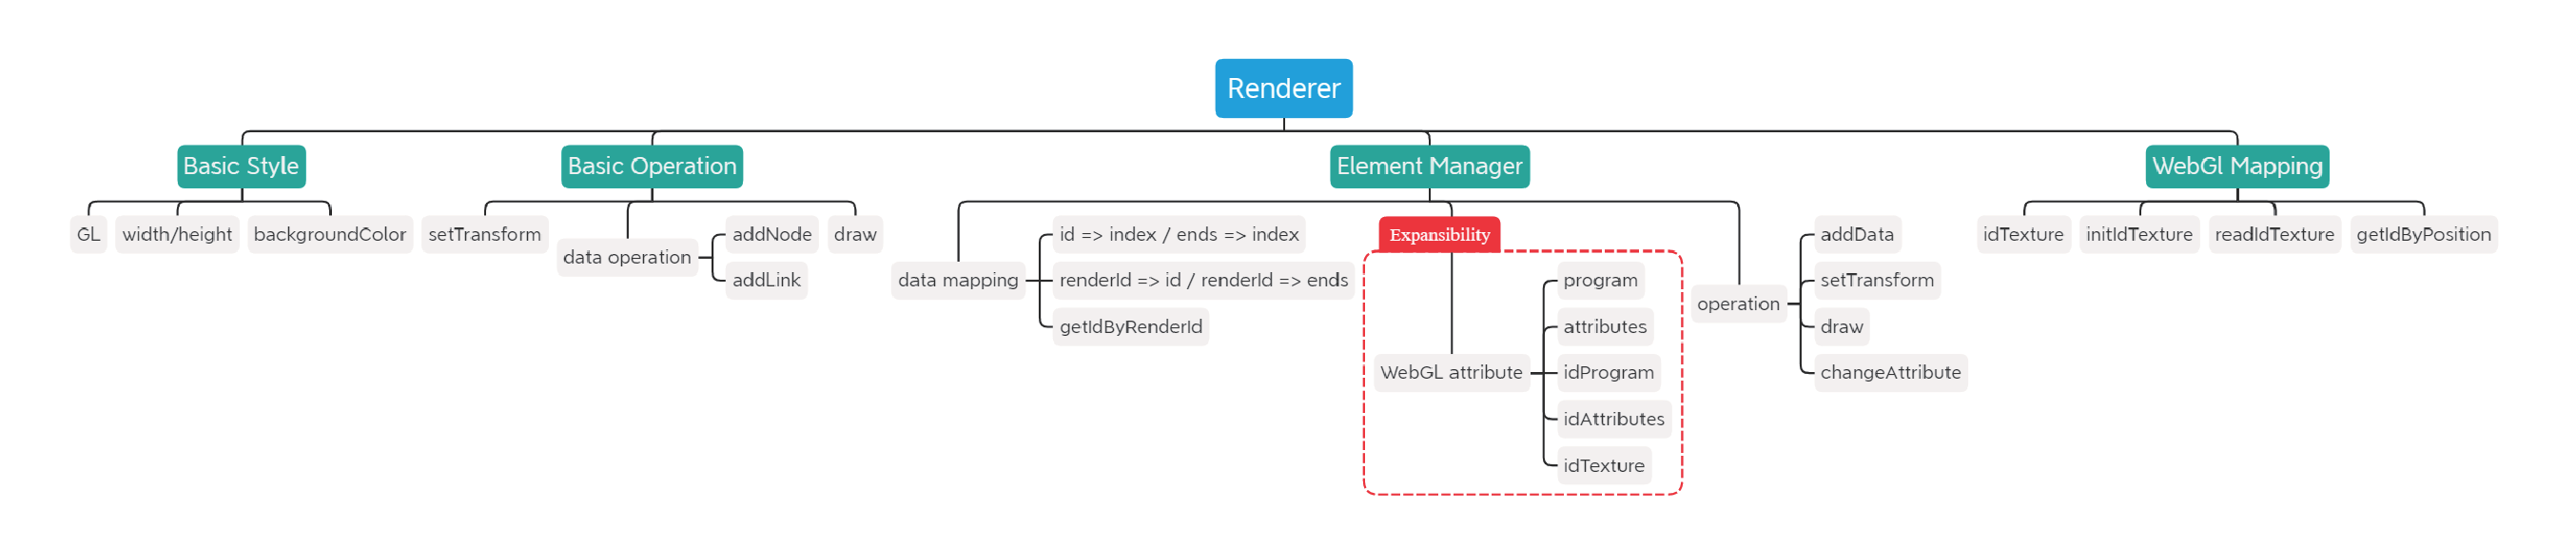
\includegraphics[width=\linewidth]{fig/xmind-01.eps}
    \caption{
        \name designs: \name consists of three parts: core engine, plugins, and library interface.
    }
    \label{fig:design}
\end{figure*}

\begin{figure}[htbp]
    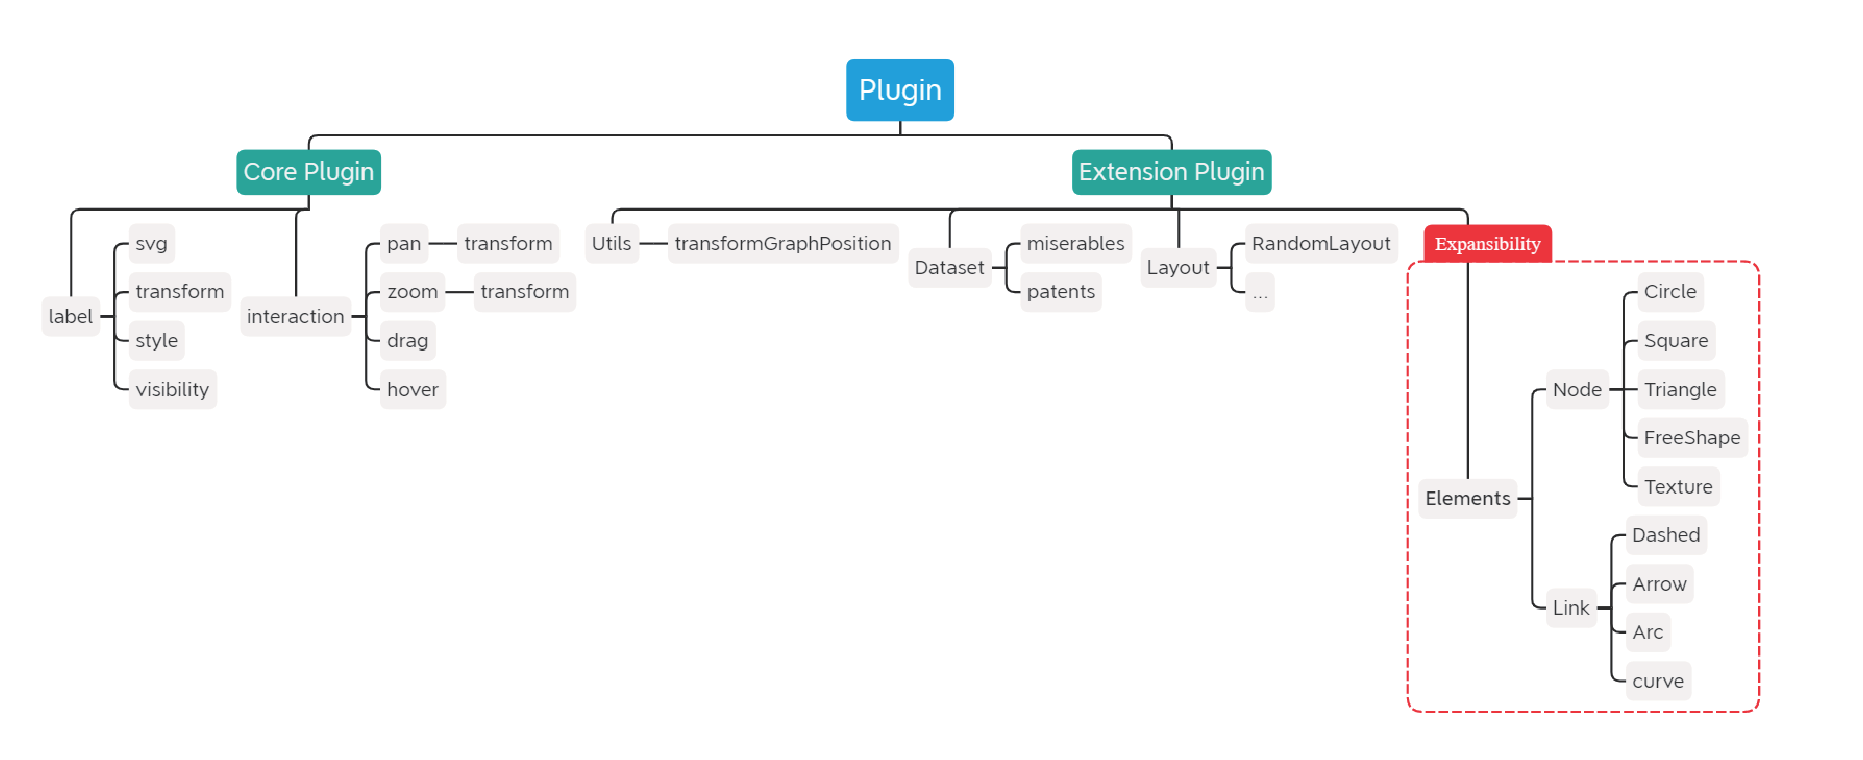
\includegraphics[width=\linewidth]{fig/xmind-02.eps}
    \caption{
        \name designs: \name consists of three parts: core engine, plugins, and library interface.
    }
    \label{fig:design}
\end{figure}
\begin{figure}[htbp]
    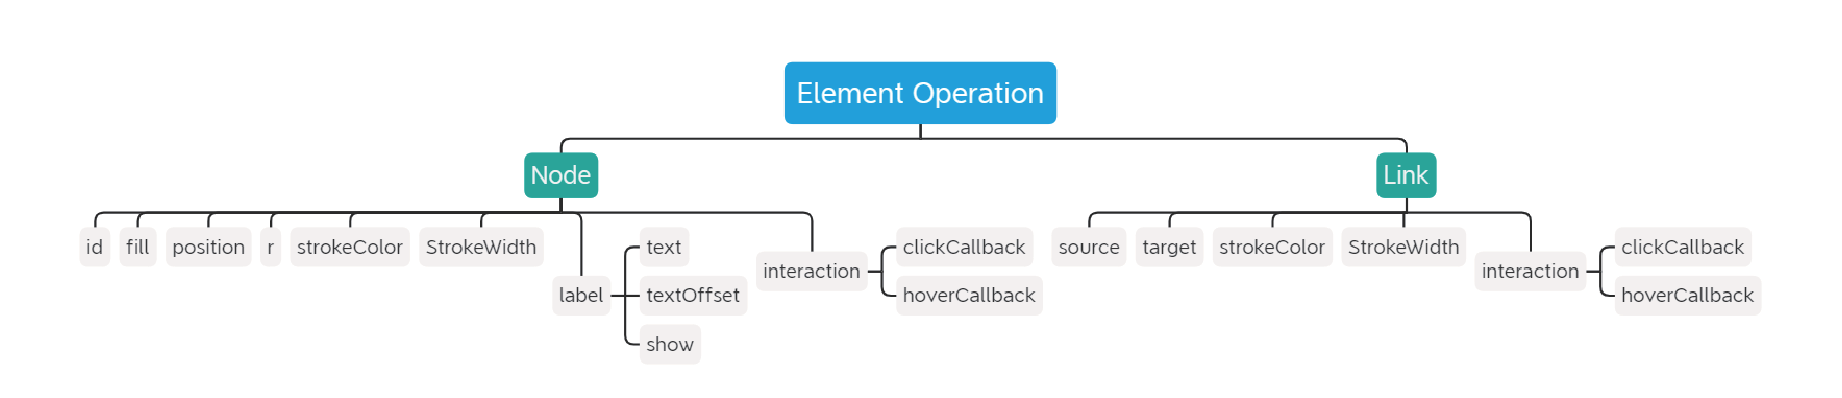
\includegraphics[width=\linewidth]{fig/xmind-03.eps}
    \caption{
        \name designs: \name consists of three parts: core engine, plugins, and library interface.
    }
    \label{fig:design}
\end{figure}
\begin{figure}[htbp]
    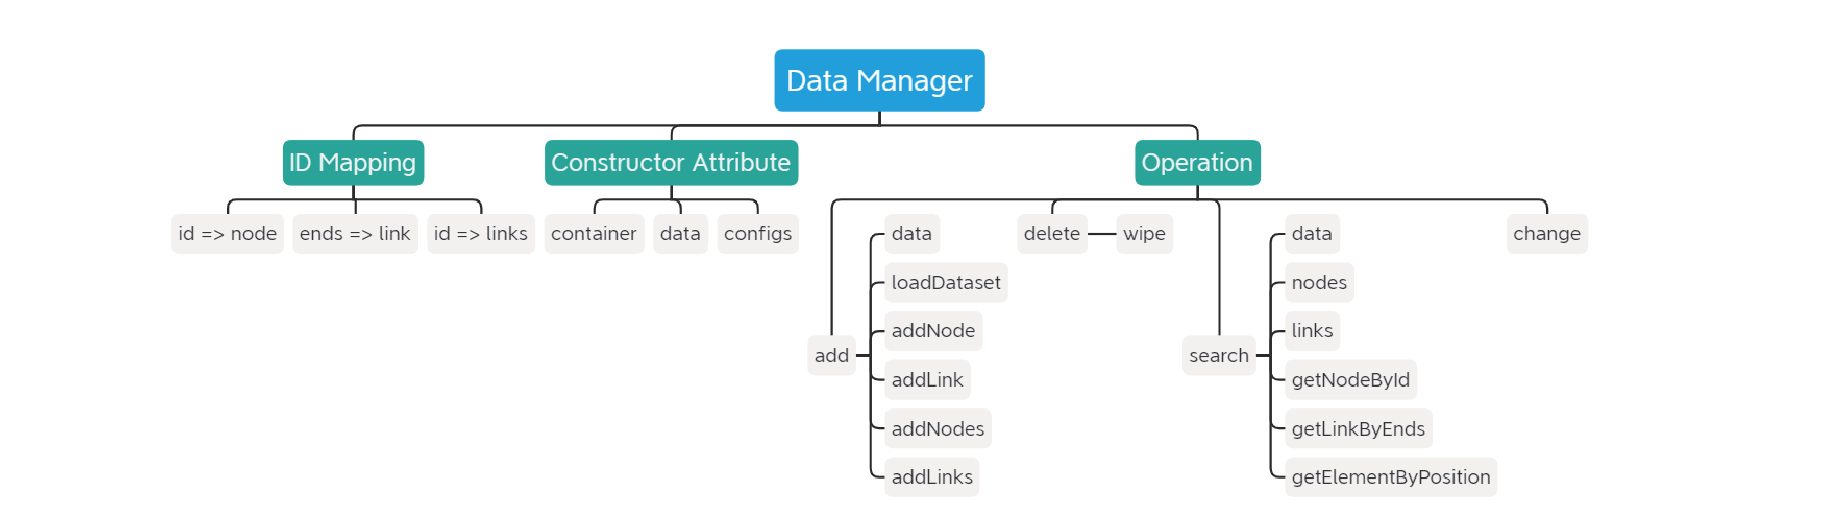
\includegraphics[width=\linewidth]{fig/xmind-04.eps}
    \caption{
        \name designs: \name consists of three parts: core engine, plugins, and library interface.
    }
    \label{fig:design}
\end{figure}

\subsection {Design Requirements of \name}

\deleted[id=pan]{为了探索\name的设计空间,我们采访了3个图可视化相关的专家,调研了一系列图可视化的工具,包括 Gephi, Cytoscape.js, Sigma.js, GraphViZ,总结了如下高性能节点链接图可视化的设计需求:}

\added[id=pan] {To explore the design space of \name, we interviewed 3 graph visualization experts, investigated 6 graph visualization tools including Gephi~\cite{DBLP:conf/icwsm/BastianHJ09}, Pajek~\cite{DBLP:reference/snam/BatageljM14}, SNAP~\cite{leskovec2016snap}, Sigma.js~\cite{DBLP:journals/jossw/Coene18}, GraphViZ~\cite{Ellson03graphvizand}, and Cytoscape.js~\cite{DBLP:journals/bioinformatics/FranzLHDSB16}. We summarized the following design requirements for high-performance node-link diagram visualization: }

\begin{itemize}
\item \deleted[id=pan]{\textbf{需要对拥有大量可视化元素的节点链接图提供高刷新率}: 根据我们对三位图可视化专家的采访,他们认为【对超过10万元素的大规模图有30fps以上的渲染速度】才能认为其对大规模节点链接图提供了高性能渲染的能力。}
\item \deleted[id=pan]{\textbf{需要有抽象的图模型来帮助控制图可视化}: 为了简化开发者对于可视化的操作,\name需要一个抽象图模型来控制图可视化而非直接控制图可视化的元素。该模型需要支持图的以下几点特性:}
\begin{itemize}
    \item \deleted[id=pan]{\textbf{链接关联节点}: }
    \item \deleted[id=pan]{\textbf{邻节点和邻接边的可访问性}: }
    \item \deleted[id=pan]{\textbf{基本图度量的计算}: }
    \item \deleted[id=pan]{\textbf{基本图论算法的支持}: }
\end{itemize}
\item \deleted[id=pan]{\textbf{支持不同节点和链接的样式}:}
\item \deleted[id=pan]{\textbf{需要提供多种布局功能和自定义布局插件}:}
\item \deleted[id=pan]{\textbf{需要提供基本的文本标签渲染和自定义标签}:}
\item \deleted[id=pan]{\textbf{需要提供基础交互模型}:}
\end{itemize}


\name aims to help users rapidly and efficiently construct network visualization applications.
Specifically, \name consists of three parts: the core engine, plugins, and library interface (\autoref{fig:design}).
The core engine contains the data manager for maintaining nodes and links and the renderer for leveraging GPU processing power to render a large-scale network.
The plugins are employed to increase and expand more requirements and functions.
The library interface aims to help developers rapidly construct applications with friendly and concise APIs.


\subsection{Core Engine}
The core engine aims to render large-scale network based on WebGL and maintains the primary network information for rapidly editing operations.
It consists of the data manager and the renderer.

\subsubsection{Data Manager}
The data manager supports a series of interface corresponding network structure.
It is used to achieve nodes or links operations, including adding, deleting, searching, and editing.
Node-links and link-nodes mapping tables are also supported for accelerating search and locate.
At the same time, the data manager has a build-in network data set for developers to get started quickly.

\subsubsection{Renderer}
The renderer aims to render basic elements: nodes and links. It focuses on the efficiency of rendering massive data on the browser platform. As the highest performance graphics rendering API of browser platform, \name uses WebGL as the bottom rendering.
However, WebGL programming is still hard and complex.
The WebGL API is encapsulate
In order to reduce the program execution time as much as possible, the basic WebGL API is only encapsulated to meet the most basic data processing and rendering.
Specifically, the renderer uses three strategies to improve rendering efficiency.

\begin{itemize}
\item \textbf{Batch}: The renderer contains a batch drawing element instance. Considering that most of the elements of the network are the same, but the location information is different. The renderer creates an instance of an element and draws it in the batch process to reduce the consuming time of the rendering process.

\item \textbf{Shader}: The renderer uses Shader function to control the shape render. Each node's shape usually needs to be defined as a circle, square, ellipse, and so on. However, the complex shape will cause a serious effect on rendering performance.
\name exploits the powerful Shader function to define and render shape in GPU with batch processing.

\item \textbf{Modify as needed}: The renderer supports manual rendering function for developers.
The main attributes of elements, including positions, color, and texture, are stored into different buffers of GPU.
When attributes of elements need to be Modified, the renderer can refresh corresponding buffers rather getting attributes from the data manager. And then, developers can refresh the network by supported function. The time consuming of getting attributes from the data manager can be omitted.

\item \textbf{Element positioning}: The renderer has an elements positioning function for supporting elements search and interaction. For improving user interaction efficiency, the renderer uses the WebGL Texture to record the screen pixel position of each element.
The time consuming of elements positioning has great improvement compared with index search and spatial index tree.
The time complexity of the function is $O(1)$.

\end{itemize}

\subsection{Plugin module}
The goal of the plugin modular is to enhance future expansions.
For supporting more features and requirements, \name designs the plugin modular to employ new improvements or functions.
At the same time, it can isolate the core modular from the rest.
For now, the plugin module includes:
\begin{itemize}
    \item \textbf{Interaction: } It supports binding interaction events and callback functions of elements. Interaction events contain basis events of edges and nodes such as Hover, MouseDown, Click, etc.
    \item \textbf{Layout: } It contains build-int layouts and allows users to use custom layouts.

\end{itemize}

\subsection{Library Interface}
The library interface aims to support concise and efficient API for users to build large-scale network visual analysis applications quickly.
Users do not need to touch the underlying WebGL rendering programming. Humanized and simple API can be called to config data and render network.
Specifically, it includes three parts:
\begin{itemize}
    \item \textbf{Global: }It is used to define custom configs, such as the mount node, the default style of the canvas, and the default style of elements.
    \item  \textbf{Element: }It includes the data adding of nodes of edges and the attributes changing of elements.
    \item  \textbf{Plugin: }It aims to set up different plugins, such as layouts and interactions.
\end{itemize}
